\section*{Bayesian teting and ``interval'' estimation}
%%%%%%%%%%%%%%%%%%%%%%%%%%%%%%%%%%%
\begin{frame}{The duality between estimation and testing}
Similarly to the frequentist case, in Bayesian inference there is an intimate relationship between testing hypotheses an estimating measurable functions of the parameters.
\begin{defn}[Test]
 Consider a statistical model $f(x \mid \theta)$  with $\theta \in \boldsymbol{\Theta}$. 
 Given $\boldsymbol{\Theta}_0 \subset \boldsymbol{\Theta}$, a \textit{test} consists in answering the question of whether
 $$ H_0 : \theta \in \boldsymbol{\Theta}_0 $$
 is true.
 We call $H_0$ the \textit{null hypothesis} and $\boldsymbol{\Theta}_0$ can often be a point, i.e. $\boldsymbol{\Theta}_0 = \{\theta_0 \}$.
\end{defn}
Notice that $\mathbb{I}_{\boldsymbol{\Theta}_0}(\theta)$ is measurable and thus we can define, for instance
\begin{equation*}
L_1(\theta, \varphi) = \begin{cases}
1, \varphi = \mathbb{I}_{\boldsymbol{\Theta}_0}(\theta),\\
0, \: \text{otherwise},
\end{cases}
\end{equation*}
which in turn leads to 
\begin{equation*}
\varphi_1 = \begin{cases}
1, \pr(\theta \in \boldsymbol{\Theta}_0 \mid x) > \pr(\theta \in \boldsymbol{\Theta}_0^c \mid x),\\
0, \: \text{otherwise}.
\end{cases}
\end{equation*}
\end{frame}
%%%%%%%%%%%%%%%%%%%%%%%%%%%%%%%%%%%
\begin{frame}{A refinement}
 The loss function just seen can be refined to
 \begin{equation*}
L_2(\theta, \varphi) = \begin{cases}
0, \varphi = \mathbb{I}_{\boldsymbol{\Theta}_0}(\theta),\\
a_0, \theta \in \boldsymbol{\Theta}_0, \varphi = 0\\
a_1, \theta \in \boldsymbol{\Theta}_0^c, \varphi = 1.
\end{cases}
\end{equation*}
Under this loss, we have
\begin{equation*}
\varphi_2 = \begin{cases}
1, \pr(\theta \in \boldsymbol{\Theta}_0 \mid x) >  a_1/(a_0 + a_1),\\
0, \: \text{otherwise}.
\end{cases}
\end{equation*}
\end{frame}
%%%%%%%%%%%%%%%%%%%%%%%%%%%%%%%%%%%
\begin{frame}{Example}
\begin{example}[\textit{One} Normal test]
  Take, for example, $x \sim \operatorname{Normal}(\theta, \sigma^2)$, with $\theta \sim \operatorname{Normal}(\mu_0, \tau^2)$.
This implies $\theta \mid x \sim \operatorname{Normal}(\mu(x), \omega^2)$, where
\begin{align*}
 \mu(x) &= \frac{\sigma^2\mu_0 + \tau^2x}{\sigma^2 + \tau^2};
 \omega^2 = \frac{\sigma^2\tau^2}{\sigma^2 + \tau^2}.
\end{align*}
To test $H_0: \theta < 0$, we can compute
\begin{align*}
 \pr(\theta < 0 \mid x) &= \pr \left(\frac{\theta-\mu(x)}{\omega} < \frac{\mu(x)}{\omega}\right), \\
 &= \Phi\left(\frac{-\mu(x)}{\omega}\right).
\end{align*}
This means that if $z_{a_0, a_1}$ is such that $\Phi(z_{a_0, a_1}) = a_1/(a_0 + a_1)$, we can accept $H_0$ if 
$$\mu(x) < -z_{a_0, a_1}\omega. $$
\end{example}
\end{frame}
%%%%%%%%%%%%%%%%%%%%%%%%%%%%%%%%%%%
\begin{frame}{Bayes factors}
A central tool in Bayesian testing is the \textbf{Bayes factor} -- see \cite{Kass1995} for a review and guide for interpretation.
\begin{defn}[Bayes factor]
 \label{def:Bayes_factor}
 The Bayes factor is the ratio of posterior odds and the prior odds over the null and the alternative:
 \begin{align*}
  B^\pi_{01}(x) &= \frac{\pr(\theta \in\boldsymbol{\Theta}_0 \mid x)}{\pr(\theta \in\boldsymbol{\Theta}_1 \mid x)}\bigg/\frac{\pr(\theta \in\boldsymbol{\Theta}_0)}{\pr(\theta \in\boldsymbol{\Theta}_1)},\\
  &= \frac{\pr(\theta \in\boldsymbol{\Theta}_0 \mid x)\cdot\pr(\theta \in\boldsymbol{\Theta}_1)}{\pr(\theta \in\boldsymbol{\Theta}_1 \mid x)\cdot\pr(\theta \in\boldsymbol{\Theta}_0)}.
 \end{align*}
\begin{remark}
 When $\boldsymbol{\Theta}_0 = \{\theta_0\}$ and  $\boldsymbol{\Theta}_1 = \{\theta_1\}$ the Bayes factor simplifies to
 \begin{equation*}
  r_{01}(x) = \frac{f(x\mid\theta_0)}{f(x\mid\theta_1)},
 \end{equation*}
 also known as the \textbf{likelihood ratio}.
\end{remark}
\end{defn}
\end{frame}
%%%%%%%%%%%%%%%%%%%%%%%%%%%%%%%%%%%
\begin{frame}{A few more considerations on the Bayes factor}
The Bayes factor can also be written as 
\begin{align*}
  B^\pi_{01}(x) &=  \frac{\int_{\boldsymbol{\Theta}_0} f(x\mid t)\pi_0(t)\,dt }{\int_{\boldsymbol{\Theta}_1} f(x\mid t)\pi_1(t)\,dt} = \frac{m_0(x)}{m_1(x)},
\end{align*}
where $\pi_0$ and $\pi_1$ are the prior distributions under each hypothesis.
Also, if $\hat{\theta}_0$ and $\hat{\theta}_1$ are the MLE under each hypothesis, by making $\pi_0$ and $\pi_1$ Dirac masses at $\hat{\theta}_0$ and $\hat{\theta}_1$, respectively, we recover
\begin{equation}
\label{eq:bayes_lrt}
 R(x) = \frac{\sup_{\theta \in \boldsymbol{\Theta}_0}f(x \mid \theta)}{\sup_{\theta \in \boldsymbol{\Theta}_1}f(x \mid \theta)}
\end{equation}
\begin{exercise}[Bayesian justifcation of LRT]
 Does (\ref{eq:bayes_lrt}) offer a Bayesian justifcation for likelihood ratios?
\end{exercise}
\end{frame}
%%%%%%%%%%%%%%%%%%%%%%%%%%%%%%%%%%%
\begin{frame}{Testing point-null hypotheses}
Hypotheses of the form $H_i : \theta \in \{ \theta_i \}$, called point-null hypotheses, are hard to deal with from a probabilistic point of view.
\begin{remark}[Point-null hypotheses under continuous priors]
 Point-null cannot be tested under continuous prior distributions.
 More generally, if either $H_0$ or $H_1$ are \textbf{impossible} \textit{a priori}, then no amount of data can change that belief.
\end{remark}
\begin{idea}[Cromwell's law\footnote{This idea is attributed to British statistician Dennis Lindley (1923-2013), one of the founders of modern Bayesian theory.}]
 In general, one not assign probability zero to events that are not logically or physically demonstrably impossible.
 Or, more eloquently, as  Oliver Cromwell writes to the General Assembly of the Church of Scotland on 3 August 1650:
 \begin{quotation}
  I beseech you, in the bowels of Christ, think it possible that you may be mistaken.
 \end{quotation}
\end{idea} 
\end{frame}
%%%%%%%%%%%%%%%%%%%%%%%%%%%%%%%%%%%
\begin{frame}{Point-null hypotheses: modification of the prior}
Testing point-null hypotheses involves a \textbf{modification of the prior}
 If $H_0: \theta \in \{\theta_0\}$  we can write $\rho_0 = \pr(\theta = \theta_0)$ and then
 \begin{equation*}
  \tilde{\pi}(\theta) = \rho_0 \mathbb{I}_{\boldsymbol{\Theta}_0}(\theta) + (1-\rho_0)\pi_1(\theta),
 \end{equation*}
is our new prior, where $\pi_1$ is the distribution with density $g_1(\theta) \propto \pi(\theta)\mathbb{I}_{\boldsymbol{\Theta}_1}(\theta)$ with respect to the dominating measure on $\boldsymbol{\Theta}_1$. 
This gives a posterior probability
\begin{equation*}
 \tilde{\pi}(\boldsymbol{\Theta}_0 \mid x) = \frac{f(x \mid \theta_0)\rho_0}{f(x \mid \theta_0)\rho_0 + (1-\rho_0)m_1(x)}.
\end{equation*}
where $m_1(x) = \int_{\boldsymbol{\Theta}_1} f(x \mid t)g_1(t)\,dt$.
It can be shown that
\begin{equation*}
 \tilde{\pi}(\boldsymbol{\Theta}_0 \mid x) = \left[1 + \frac{1-\rho_0}{\rho_0}\frac{1}{B^\pi_{01}(x)}\right]^{-1}, 
\end{equation*}
which makes clear the relationship between posterior probabilities and Bayes factors.
\end{frame}
%%%%%%%%%%%%%%%%%%%%%%%%%%%%%%%%%%%
\begin{frame}{Example}
Consider $x \sim \operatorname{Binomial}(n, p)$ and consider testing $H_0: p = 1/2$ against $H_1: p \neq 1/2$. 
Taking $g_1(p) = 1$, we have
\begin{equation*}
  \tilde{\pi}(\boldsymbol{\Theta}_0 \mid x) = \left[1 + \frac{1-\rho_0}{\rho_0}2^n B(x+1, n-x+1)\right]^{-1}.
\end{equation*}
 \begin{center}
 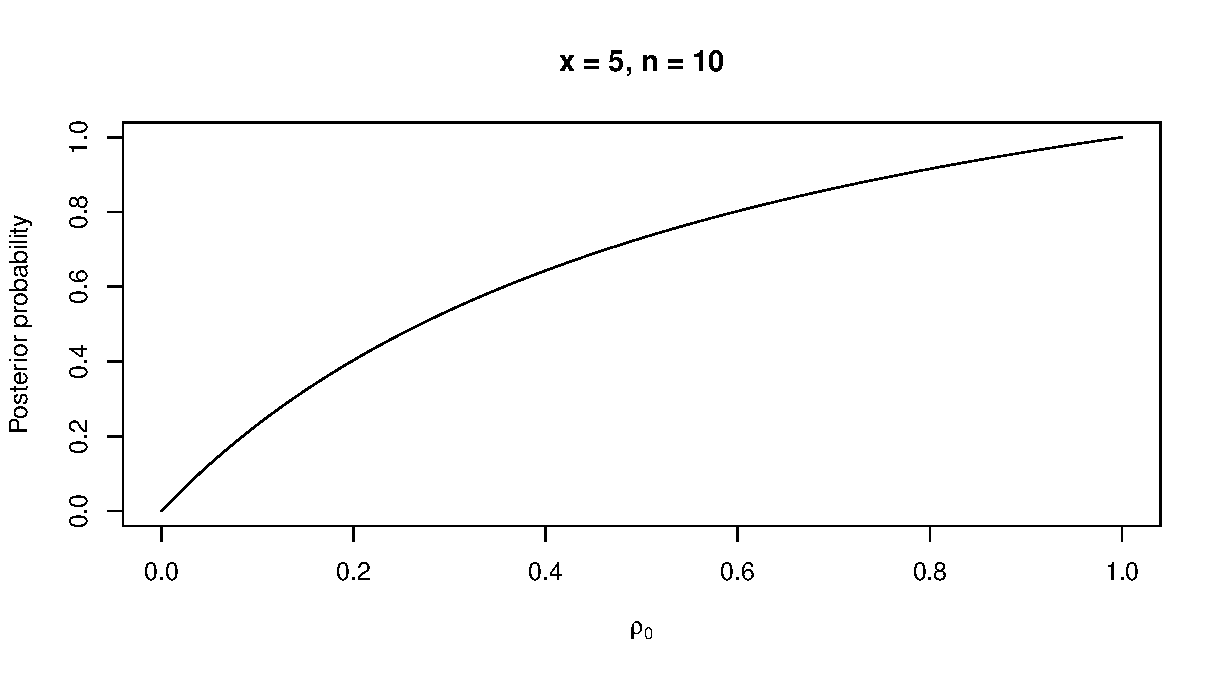
\includegraphics[scale=0.45]{figures/posterior_prob_half.pdf}
\end{center}
\end{frame}
%%%%%%%%%%%%%%%%%%%%%%%%%%%%%%%%%%%
\begin{frame}{Testing with improper priors}
 \begin{idea}[Bayesian hypothesis testing with improper priors]
  No. Just... No.
 \end{idea}
See~\cite{Degroot1973} for the many reasons why this is just a bad idea.
If you insist, please see Section 5.2.5 in \cite{Robert2007} and references therein.
\end{frame}
%%%%%%%%%%%%%%%%%%%%%%%%%%%%%%%%%%%
\begin{frame}{An interesting little paradox}
\begin{idea}[The Jeffreys-Lindley paradox]
Consider $x \sim \operatorname{Normal}(\theta, \sigma^2)$ with $\sigma^2$ known and suppose we are interested in testing $H_0: \theta = \theta_0$ against $H_1: \theta \neq \theta_0$.
We can summarise the data using the sample mean $\bar{x}$ and then compute $t_n = \sqrt{n}(\bar{x}-\theta_0)/\sigma$. 
Employing a conjugate prior $\theta \sim \operatorname{Normal}(\mu_0, \sigma^2)$,
the Bayes factor is
\begin{equation*}
B_{01}(\boldsymbol{x}) = \sqrt{1 + n}\exp\left(-\frac{nt_n^2}{2(1+n)}\right),
\end{equation*}
which goes to infinity with $n$, while the p-value:
\begin{equation*}
 p(t_n) = 1-2\Phi(|t_n|),
\end{equation*}
is constant in $n$.
In practice this means that, for instance $t_n = 1.96$ and $n = 16, 818$, we have 95\% frequentist confidence that $\theta \neq \theta_0$ whilst \textbf{at the same time} having 95\% belief that $\theta = \theta_0$.
\end{idea} 
\end{frame}
%%%%%%%%%%%%%%%%%%%%%%%%%%%%%%%%%%%
\begin{frame}{Another look at principled Bayesian testing}
 Before we were doing
 \begin{equation*}
  L_3(\theta, \varphi) = |\varphi - \mathbb{I}_{\boldsymbol{\Theta}_0}(\theta)|.
 \end{equation*}
But considering a strictly convex loss such as the quadratic loss 
 \begin{equation*}
  L_4(\theta, \varphi) = \left(\varphi - \mathbb{I}_{\boldsymbol{\Theta}_0}(\theta)\right)^2,
 \end{equation*}
 leads to better (more adaptable) estimators in general.
 For instance, the Bayes estimator under $L_4$ is
 \begin{equation*}
  \varphi_\pi(x) = \pr(\theta \in  \boldsymbol{\Theta}_0 \mid x).
 \end{equation*}
 \end{frame}
%%%%%%%%%%%%%%%%%%%%%%%%%%%%%%%%%%%
\begin{frame}{Credibility regions}
After all of this work, we are finally ready to define credibility regions, the main object in Bayesian interval estimation.
\begin{defn}[Credibility region]
For a prior $\pi$, a set $C_x$ is called an $\alpha$-credible set if 
\begin{equation*}
 \pr(\theta \in C_x \mid x) \geq 1-\alpha.
\end{equation*}
We call $C_x$ a highest posterior density (HPD) $\alpha$-credible region if
\begin{equation*}
 \left\{\theta : p(\theta \mid x) > k_\alpha \right\} \subset C_x \subset \left\{\theta : p(\theta \mid x) \geq k_\alpha \right\},
\end{equation*}
subject to the restriction that
\begin{equation*}
 \pr(\theta \in C_x^\alpha) \geq 1-\alpha.
\end{equation*}
\end{defn}
\end{frame}
%%%%%%%%%%%%%%%%%%%%%%%%%%%%%%%%%%%
\begin{frame}{A couple remarks}
Credibility regions have a few desirable properties that make them quite attractive as ``interval'' estimates.
\begin{remark}[No randomisation]
 One nice feature of credibility regions for discrete distributions is that, contrary to the frequentist approach, no randomisation is needed to attain a certain level $\alpha$.
\end{remark}
Also,
\begin{remark}[Improper priors and credibility regions]
 In principle, the use of improper priors poses no problem for the derivation of credibility regions.
\end{remark} 
\end{frame}
%%%%%%%%%%%%%%%%%%%%%%%%%%%%%%%%%%%
\begin{frame}{Credibility regions: Example I}
Sometimes we will be able to provide Bayesian justifcation for frequentist confidence regions/intervals.
\begin{example}[Credibility intervals for the variance in the Normal]
\label{ex:cred_var_normal_Jeffreys}
Consider $\boldsymbol{x} = \{ x_1, \ldots, x_n \}$, $x_i \sim \operatorname{Normal}(\theta, \sigma^2)$, with both parameters unknown.
Consider
$$ \pi(\theta, \sigma^2) \propto \frac{1}{\sigma^2}. $$
Make $s^2 = \sum_{i=1}^n (x-\bar{x})^2$.
It can be shown that $p(\sigma^2 \mid  s^2) \equiv \operatorname{Gamma}(\sigma^2; (n-1)/2, s^2/2)$.
In particular, this implies
\begin{equation*}
 \frac{s^2}{\sigma^2} \mid \bar{x} \sim \operatorname{Chi-square}(n-1),
\end{equation*}
which the attentive student will notice leads to the same solution as the classical confidence approach.
\end{example}
\end{frame}
%%%%%%%%%%%%%%%%%%%%%%%%%%%%%%%%%%%
\begin{frame}{Credibility regions: Example II}
\begin{example}[HPD for the normal mean]
\label{ex:cred_mean_normal_Jeffreys}
 Consider again the setting of example~\ref{ex:cred_var_normal_Jeffreys}.
 Define $\bar{s}^2 = s^2/(n-1)$ and take $t = F_{\text{Student}}^{-1}(\alpha; n-1)$.
 The classical ``T'' interval,
 \begin{equation*}
  C_t(\bar{x}, \bar{s}^2) = \left(\bar{x} - t\sqrt{\frac{\bar{s}^2}{n}}, \bar{x} + t\sqrt{\frac{\bar{s}^2}{n}}\right),
 \end{equation*}
 is a HPD region under the Jeffreys's prior.
 Again, we can show that
 \begin{equation*}
  \sqrt{n}\frac{\theta -\bar{x}}{\sqrt{\bar{s}^2}} \mid \bar{x}, \sqrt{\bar{s}^2} \sim \operatorname{Student-t}(n-1).
 \end{equation*}
\end{example}
 
\end{frame}
%%%%%%%%%%%%%%%%%%%%%%%%%%%%%%%%%%%
\begin{frame}{A little decision theory can't hurt... Or can it?}
 Consider the loss
 \begin{equation*}
  L_1(C, \theta) = \operatorname{vol}(C) + (1-\mathbb{I}_{C}(\theta))a,
 \end{equation*}
 which leads to the risk
 \begin{equation*}
  R(C_x, \theta) = E[\operatorname{vol}(C_x)] + \pr(\theta \notin C_x).
 \end{equation*}
Under this loss, the interval in Example~\ref{ex:cred_mean_normal_Jeffreys} is dominated by 
\begin{equation*}
 C_t^\prime(\bar{x}, \bar{s}^2) = \begin{cases}
C_t(\bar{x}, \bar{s}^2), \sqrt{\bar{s}^2} < \sqrt{n}c/(2t),\\
\{\bar{x}\}, \: \text{otherwise},
\end{cases}
\end{equation*}
which is a bit weird -- why?

Now, consider what happens under a \textit{rational loss}
\begin{equation*}
 L_k(C, \theta) = \frac{\operatorname{vol}(C)}{\operatorname{vol}(C) + k} + (1-\mathbb{I}_{C}(\theta)), k >0.
\end{equation*}
\end{frame}
%%%%%%%%%%%%%%%%%%%%%%%%%%%%%%%%%%%
\begin{frame}{HPD (or HDI in one dimension)}
 \begin{center}
 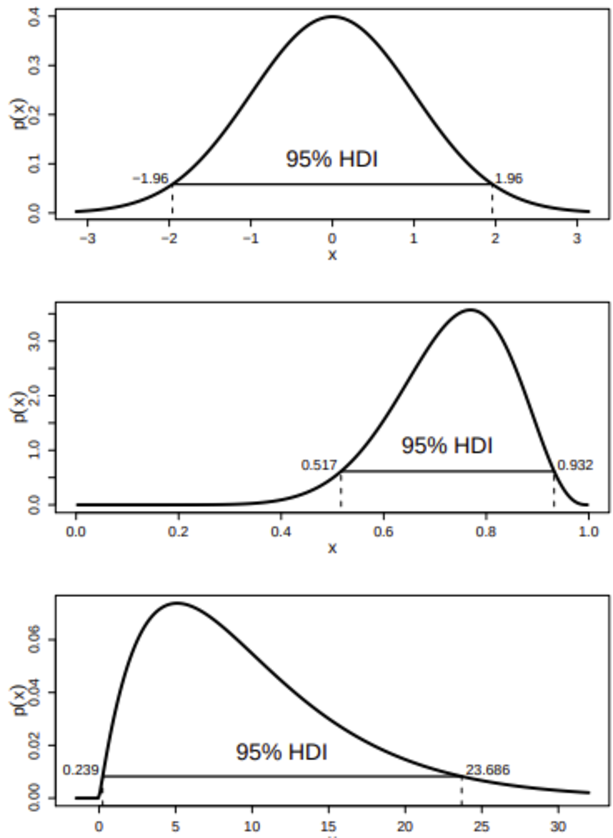
\includegraphics[scale=0.5]{figures/HDI.pdf}
\end{center}
\end{frame}
%%%%%%%%%%%%%%%%%%%%%%%%%%%%%%%%%%%
\begin{frame}{Recommended reading}
\begin{itemize}
  \item[\faBook] \cite{Robert2007}, Ch. 5.
%  \item 
 \item[\faForward] Next lecture: \cite{Robert2007} Ch. 7.
 \end{itemize} 
\end{frame}
